% Chapter mq, part D: the Thorin side of (M). Sources: misc/reviews/nick-inequality-M-thorin/inequality_M_thorin_chapter_for_vadim/chapter_inequality_M_thorin.tex (Sections on the explicit formula, hitting times, the resolvent family, the duality, the ladder), misc/reviews/nick-line-towards-M-v2/line_towards_M_for_vadim/chapter_line_of_proof_M.tex (reciprocal scale, helix, Stieltjes fraction, finite field circle), misc/reviews/nick-merge-additions/merge_additions_for_vadim/chapter_hitting_wald_M.tex; referee reports misc/research/directions/opus/vol3/MT.md, ML2.md, MW.md; numbers and figures misc/vol3/verify/MQFIG/thorin.md and line.md; edited 23 Nov 2026.
\section{The Thorin side of (M)}\label{mqt:sec:main}

This part collects the discussion of the Chebyshev statistic in the language of Thorin measures, hitting times and Esscher tilts, with the figures that go with it. Most of the mathematics is already proved in the book, in a different chart, and the sections below cite the proofs; what this part adds is the reading of a few statements in this language (the Brownian kernel of Section~\ref{mq:sec:brownian} as a duality, the Wald couple, the Esscher form of the criterion, the Stieltjes fraction, the finite field circle) and a set of computations. Everything only computed is called an observation, and is stated with its grid or its precision. Nothing in this part proves the inequality (M), and nothing in it depends on the unverified claim of a proof of RH that Part A describes.

\paragraph{Conventions.} We keep the notation of Section~\ref{mq:sec:setting}: $\mathcal G$ is the Riesz mean, $F_0=2+\gamma_E-\log4\pi=0.0461914$, $\mathrm{tr}$ is the trivial zero term, and the slack is $\Phi(u)=F_0-\big(\mathcal G(e^u)-\log2\pi+\mathrm{tr}(e^u)\big)e^{-u/2}$ with $\Phi(0)=0$, the function $\Phi_{1/2}$ of Section~\ref{mq:sec:brownian}. The clock $T$ of the book has $\mathbb E\,e^{-uT}=\xi(\frac12)/\xi(\frac12+\sqrt u)$ for $u\ge0$ (Theorem~\ref{thm:ch12:idsd}, which holds unconditionally), and we put $\tau=2T$, so that $\mathbb E\,e^{-s\tau}=\xi(\frac12)/\xi(\frac12+\sqrt{2s})$ and the rates of $\tau$, when they exist, are $\lambda_\gamma=\gamma^2/2$. Sums over $\gamma>0$ run over the positive ordinates with multiplicity; without RH they run over one zero from each pair $\rho,1-\rho$, with $\gamma=-i(\rho-\frac12)$ and conjugate terms grouped, and a bare sum $\sum_\gamma$ runs over both signs of $\gamma$. We keep the chart with atoms at $\lambda_\gamma=\gamma^2/2$; the book's chart has atoms at $\gamma^2$.

\subsection{The slack and the sharp constants}\label{mqt:sub:slack}

The explicit formula \eqref{qt:eq:riesz} gives the slack as a $2\sin^2$ transform of the zero measure,
\[
\Phi(u)=\sum_{\gamma>0}\frac{2}{\frac14+\gamma^2}\,2\sin^2\Big(\frac{\gamma u}2\Big)\qquad\text{under RH,}
\]
which is equation~\eqref{st:eq:phisin}; without RH the same sum holds with $\sin^2(u\sqrt{z_\rho/2})$ at the points $z_\rho=\gamma_\rho^2/2$ of the zero measure (a Thorin measure only under RH). Landau's theorem (Proposition~\ref{qt:prop:riesz}) says that a bound $\mathcal G(x)\le Cx^\theta$ forces $\zeta\ne0$ for $\Re s>\theta$ with $\frac12\le\theta<1$, so that RH is equivalent to $\Phi\ge0$ (Theorem~\ref{st:thm:phi}), to $\mathcal G(x)\le Cx^{1/2}$, and to the sharp form $\mathcal G(x)\le\log2\pi+F_0\sqrt x-\mathrm{tr}(x)$ for all $x>1$. Under RH $\limsup(\mathcal G(x)-\log2\pi)/\sqrt x=F_0$ (Theorem~\ref{qt:thm:sharp}), because $H(u)=F_0-\Phi(u)$ is almost periodic with mean zero and $H(0)=F_0$, and $\liminf H\in[-F_0,0)$. Unconditionally, one certified range of $\Phi>0$ is $0<u\le104.86604$, that is $x\le3.4893\cdot10^{45}$, from $300$ zeros (Theorem~\ref{st:thm:cert}); it uses \cite{HSW22} with the verification of RH to height $3\cdot10^{12}$ \cite{PT21}.

\begin{figure}[htbp]
\centering
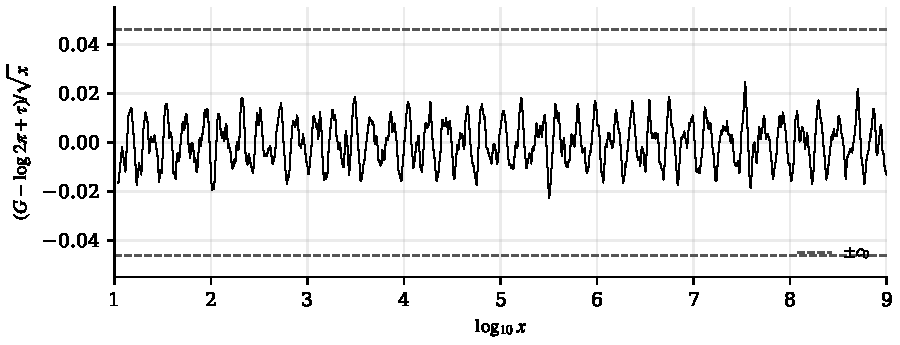
\includegraphics[width=0.95\textwidth]{fig/mq_G_primes.pdf}
\caption{The normalised Chebyshev error $(\mathcal G(x)-\log2\pi+\mathrm{tr}(x))/\sqrt x$, computed from the primes at $274000$ sampled points of $10<x\le10^9$, stays inside the barrier $\pm F_0=\pm0.0462$ (dashed); its sampled extremes are $0.0247$ (near $x=3.4186\cdot10^7$) and $-0.0227$ (at $x=319439$).}\label{mqt:fig:Gprimes}
\end{figure}

\begin{remark}[Observation]
On the $274000$ sampled points of $10<x\le10^9$ the normalised statistic lies in $[-0.02268,\,0.02469]$ (Figure~\ref{mqt:fig:Gprimes}), the largest value being about $53$ per cent of the barrier $F_0$. The supremum is approached slowly: the first ten ordinates carry $58.6$ per cent of the weight $\sum_{\gamma>0}2/(\frac14+\gamma^2)=F_0$ (Figure~\ref{mqt:fig:Klaw}).
\end{remark}

Figure~\ref{mqt:fig:Goverlay} shows the statistic as a sum over primes and as a sum over zeros: the two agree to $1.7\cdot10^{-6}$ with $20000$ ordinates. See Figure~\ref{mqt:fig:Phi}.

\begin{figure}[htbp]
\centering
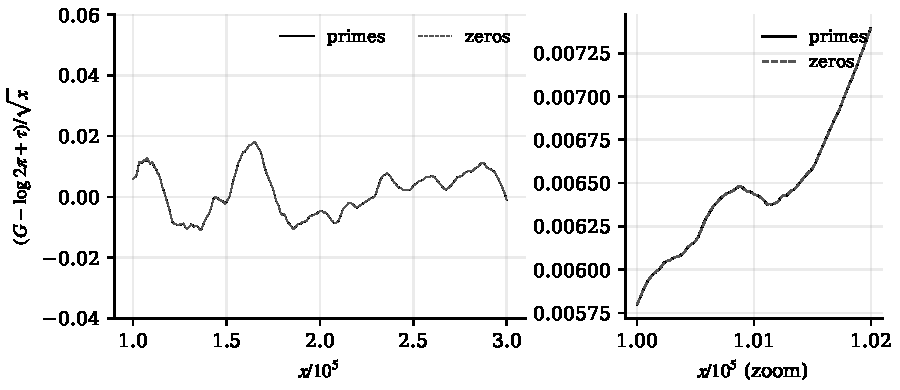
\includegraphics[width=0.95\textwidth]{fig/mq_G_overlay.pdf}
\caption{Primes (solid) against the sum over the first $20000$ ordinates (dashed grey) for the normalised statistic on $[10^5,3\cdot10^5]$: the two curves cannot be told apart (sampled largest difference $1.7\cdot10^{-6}$, root mean square $3.9\cdot10^{-7}$), the right panel enlarging $[100000,102000]$.}\label{mqt:fig:Goverlay}
\end{figure}

\begin{figure}[htbp]
\centering
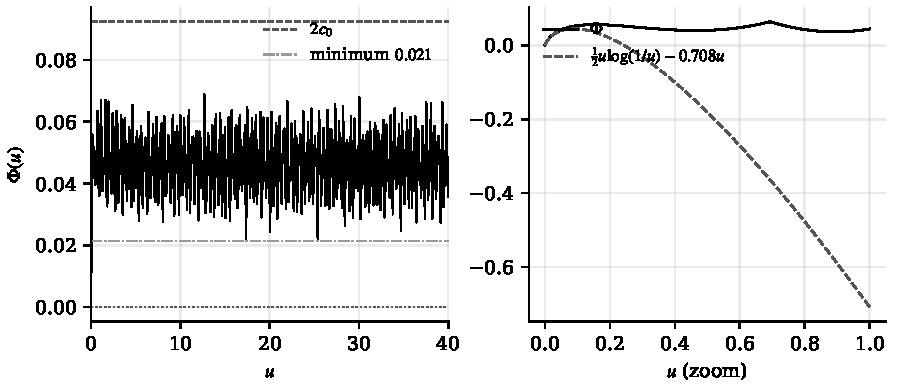
\includegraphics[width=0.95\textwidth]{fig/mq_Phi.pdf}
\caption{The Chebyshev slack $\Phi(u)$ from $20000$ zeros. Its minimum on $[0.05,40]$ is $0.0213$, at $u=25.38$ (dash dotted), and its maximum is $0.0689$ at $u=12.67$; the omitted weight of the zero sum is $F_0-\sum_{j\le20000}2/(\frac14+\gamma_j^2)=1.6\cdot10^{-4}$, which under RH bounds the cosine tail uniformly. Right: $\Phi$ near $0$ against the asymptote $\frac12u\log(1/u)-0.7075\,u$ of Proposition~\ref{mql:prop:helixprime}.}\label{mqt:fig:Phi}
\end{figure}

\subsection{The resolvent family, the $2\sin^2$ duality and the Brownian kernel}\label{mqt:sub:duality}

Section~\ref{mq:sec:brownian} gives the family $W_a$, $\Phi_a$, $c(a)=\frac1a\frac{\xi'}\xi(\frac12+a)$ and the criterion at every width $a>\frac12$ (Proposition~\ref{mq:prop:crit}; Theorem~\ref{st:thm:phi} at $a=\frac12$, the slack of the previous subsection), and $a\to0$ gives $c(0^+)=\sum_{\gamma>0}2/\gamma^2$. The constants hardly move with $a$ (Figure~\ref{mqt:fig:cofa}), because the weights $(a^2+\gamma^2)^{-1}$ change little once $\gamma\ge14$: $c(0^+)=0.04621$, $c(\frac12)=F_0=0.046191$, $c(3)=0.045563$. Figure~\ref{mqt:fig:family} shows the statistics $H_a(\log x)=c(a)-\Phi_a(\log x)$ from the primes for $a=0.25,\,0.75,\,1,\,2$ and $x\le10^7$: the four curves are almost the same.

\begin{figure}[htbp]
\centering
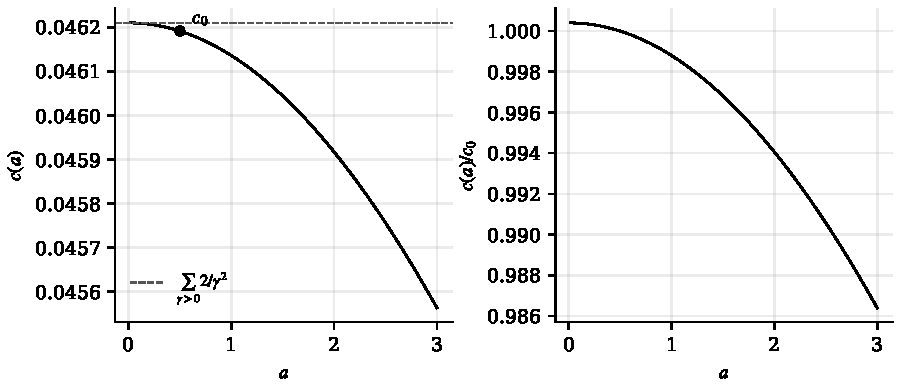
\includegraphics[width=0.95\textwidth]{fig/mq_c_of_a.pdf}
\caption{The constant $c(a)=\frac1a\frac{\xi'}\xi(\frac12+a)$ of the resolvent family, and its ratio to $F_0$; the dashed line is the limit $0.0462100$ as $a\to0$.}\label{mqt:fig:cofa}
\end{figure}

\begin{figure}[htbp]
\centering
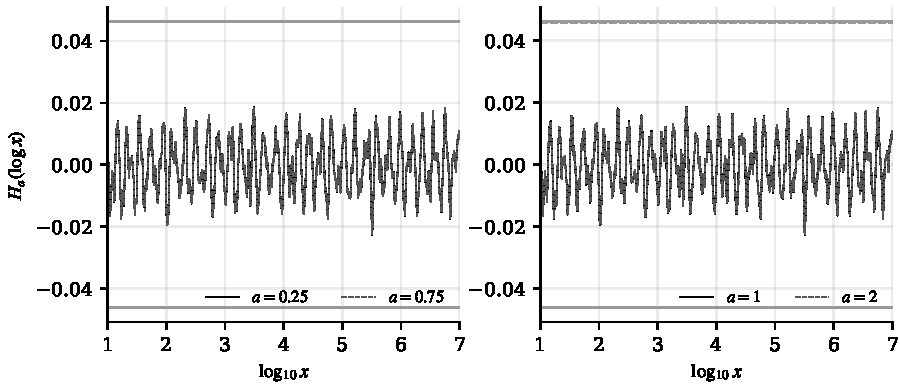
\includegraphics[width=0.95\textwidth]{fig/mq_duality_family.pdf}
\caption{The resolvent statistics $H_a(\log x)$ from primes for $a=0.25,0.75$ (left) and $a=1,2$ (right), with the barriers $\pm c(a)$; the sampled slack stays above $0.0274$ for $x\le10^7$.}\label{mqt:fig:family}
\end{figure}

The prime form of Corollary~\ref{mq:cor:primeslack} has a mirror image, which we state as a duality between a prime side and a zero side. For $a>\frac12$ and $\sigma=\frac12+a$ put
\[
C^{(a)}(t)=\sum_n\Lambda(n)\,n^{-\sigma}\,2\sin^2\Big(\frac t2\log n\Big),
\]
which converges for $a>\frac12$; $A_\sigma(t)$ is the archimedean term of Section~\ref{mq:sec:ladder}.

\begin{proposition}[The $2\sin^2$ duality]\label{mqt:prop:duality}
\begin{enumerate}
\item (Prime side.) For $a>\frac12$ the function $C^{(a)}$ is a L\'evy exponent: for every $s>0$, $e^{-sC^{(a)}(t)}$ is the characteristic function of a symmetric compound Poisson law with L\'evy measure $s\nu$, where $\nu=\frac12\sum_n\Lambda(n)n^{-\sigma}(\delta_{\log n}+\delta_{-\log n})$ is the L\'evy measure per unit time of the process with exponent $C^{(a)}$. Without hypothesis, $C^{(a)}(t)=\sum_\rho\Re\big[\frac1{\sigma+it-\rho}-\frac1{\sigma-\rho}\big]-A_\sigma(t)$ (the series of differences converges absolutely), and under RH the zero sum equals $\pi(P_a(t)-P_a(0))$ with $P_a(t)=\frac1\pi\sum_\gamma\frac a{a^2+(t-\gamma)^2}$ the Poisson smoothing of width $a$ of the zero counting measure over both signs of $\gamma$, so that $C^{(a)}(t)=\pi[P_a(t)-P_a(0)]-A_\sigma(t)$.
\item (Zero side.) For every $a>0$ outside $\{\frac52,\frac92,\dots\}$, $\Phi_a$ is a L\'evy exponent if and only if RH holds. Under RH, $e^{-s\Phi_a}$ is the characteristic function at time $s$ of the compound Poisson process with rate $c(a)$ and jump law $\pm\gamma_{K_a}$, with $K_a$ of Proposition~\ref{mq:prop:sizebias}.
\item (Exchange rule.) With $k_a(y)=e^{-a|y|}=\mathbb E\,e^{-\frac{a^2}2\eta_y}$ in the log scale $y$ ($\eta_y$ the Brownian passage time to level $|y|$) and $p_a(r)=a/[\pi(a^2+r^2)]$, convolution with $k_a$ corresponds to multiplication by the weight $2\pi p_a(r)=\frac{2a}{a^2+r^2}$ in the frequency $r$, and multiplication by $k_a$ to Poisson smoothing of width $a$. Multiplication by $2\sin^2(\frac{ty}2)$ on one side is minus one half the second difference with step $t$ on the other.
\end{enumerate}
\end{proposition}

\begin{proof}
(1) $C^{(a)}(t)=\int(1-\cos ty)\,\nu(dy)$ with $\nu\ge0$ finite, the form of Lévy and Khintchine of a compound Poisson exponent. The zero form is $\Re[\frac{\zeta'}\zeta(\sigma+it)-\frac{\zeta'}\zeta(\sigma)]$ rewritten with $\frac{\xi'}\xi(s)=\frac1s+\frac1{s-1}-\frac12\log\pi+\frac12\psi(\frac s2)+\frac{\zeta'}\zeta(s)$ and Hadamard's product in the form of a difference of logarithmic derivatives, $\frac{\xi'}\xi(\sigma+it)-\frac{\xi'}\xi(\sigma)=\sum_\rho\big[\frac1{\sigma+it-\rho}-\frac1{\sigma-\rho}\big]$, which converges absolutely; under RH each term is $\frac a{a^2+(t-\gamma)^2}-\frac a{a^2+\gamma^2}$.
(2) A continuous real negative definite function vanishing at $0$ is nonnegative, so a L\'evy exponent $\Phi_a$ satisfies $\Phi_a\ge0$, and RH follows from Proposition~\ref{qt:prop:laplace}: with the zero sum defining $W_a$ it gives $2aW_a=D_a+T_a$ with $T_a$ bounded, so that $\Phi_a\ge0$ bounds $D_a$ above and the proposition at $\theta=\frac12$ gives RH (for $a>\frac12$ this is Proposition~\ref{mq:prop:crit}, and Theorem~\ref{st:thm:phi} covers $a=\frac12$). Under RH, $\Phi_a(u)=\int(1-\cos ur)\,\nu_a(dr)$ with the finite positive measure $\nu_a$ of Proposition~\ref{mq:prop:sizebias} (and at $a=\frac12$ Theorem~\ref{st:thm:pd}), of total mass $c(a)$, which gives the stated compound Poisson law.
(3) $\int e^{-a|y|}e^{iry}dy=\frac{2a}{a^2+r^2}=2\pi p_a(r)$, so that with $\hat f(r)=\int f(y)e^{iry}dy$ we have $\widehat{k_a*f}=2\pi p_a\hat f$ and $\widehat{k_af}=p_a*\hat f$, and $\widehat{(1-\cos t\,\cdot)\mu}=\hat\mu-\frac12(\hat\mu(\cdot+t)+\hat\mu(\cdot-t))$.
\end{proof}

The two sides are mirror images with one asymmetry. The prime exponent is a L\'evy exponent for free, because primes are counted with positive weights, but it converges only for $a>\frac12$; the zero exponent exists for every $a>0$ but is a L\'evy exponent only under RH. The explicit formula exchanges them: $C^{(a)}$ at frequency $t$ is a Poisson smoothed zero count, and $\Phi_a$ at log scale $u$ is a Brownian smoothed prime count. Under RH a pairing identity follows from Tonelli, for $a>\frac12$ and $b>0$, with the sum over both signs of $\gamma$: $\sum_\gamma C^{(a)}(\gamma)/(b^2+\gamma^2)=\sum_n\Lambda(n)n^{-1/2-a}\Phi_b(\log n)$. Also under RH the $N$th cumulant of the tilted time $\mathcal T_a$ of Section~\ref{mq:sec:brownian} is $(N-1)!\sum_{\gamma>0}(2/(a^2+\gamma^2))^N$, and for $N=1$ it is $c(a)$.

The Brownian kernel of Corollary~\ref{mq:cor:primeslack} is $\kappa_a(u,y)=2e^{-ay}-e^{-a|u-y|}-e^{-a(u+y)}$, and its sign change at $y^*(u)=\frac1{2a}\log(2e^{au}-1)$ is the content of the remark that prime powers below about $\sqrt x$ lower the slack and those above raise it (Figure~\ref{mqt:fig:Dkernel}). Under RH the law of the size biased index $K=K_{1/2}$ of Proposition~\ref{mq:prop:sizebias}, $\mathbb P(K=\gamma_j)=2/(F_0(\frac14+\gamma_j^2))$, puts $0.2164$ on $\gamma_1=14.13$, $0.5860$ on the first ten ordinates and $0.99658$ on the first $20000$ (Figure~\ref{mqt:fig:Klaw}).

\begin{figure}[htbp]
\centering
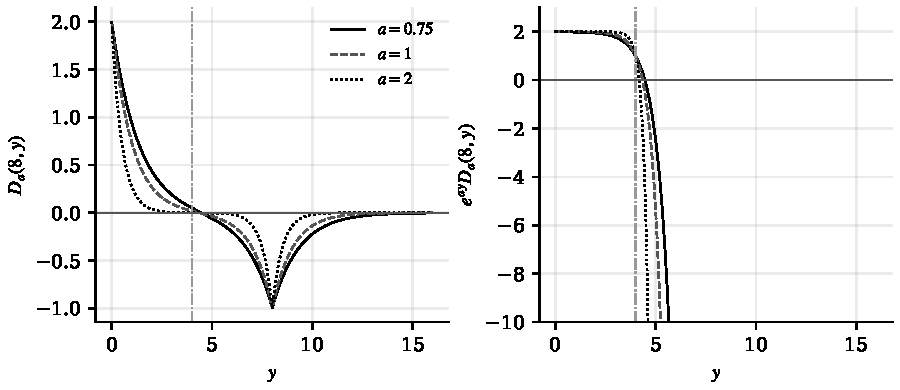
\includegraphics[width=0.95\textwidth]{fig/mq_D_kernel.pdf}
\caption{The second difference $\kappa_a(u,y)$ of the Brownian passage kernel at $u=8$ for $a=0.75,1,2$ (right: the same multiplied by $e^{ay}$). It changes sign just above $y=u/2$ (dash dotted): prime powers below about $\sqrt x$ lower the slack and those above raise it.}\label{mqt:fig:Dkernel}
\end{figure}

\begin{figure}[htbp]
\centering
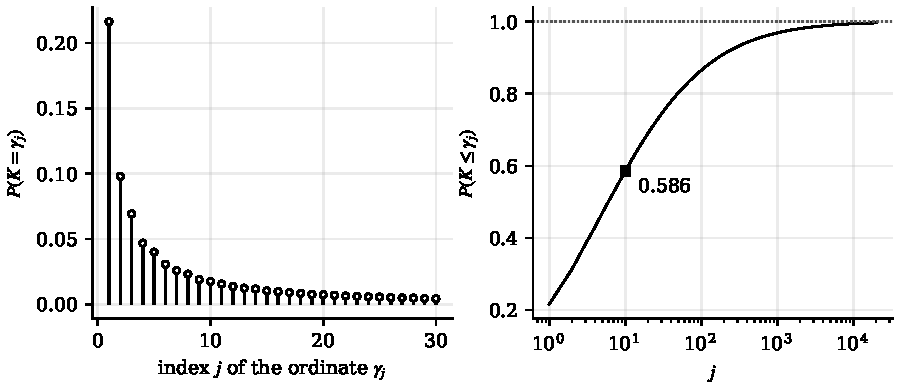
\includegraphics[width=0.95\textwidth]{fig/mq_K_law.pdf}
\caption{The law of the size biased index $K$ (under RH). Left: $\mathbb P(K=\gamma_j)$ for the first $30$ ordinates; right: its distribution function against $j$ (logarithmic scale), which reaches $0.586$ at $j=10$.}\label{mqt:fig:Klaw}
\end{figure}

\subsection{The reciprocal scale, complete monotonicity and Gamma probes}\label{mqt:sub:reciprocal}

On the reciprocal scale no individual ordinate is seen. The Laplace transform $\hat\Phi(b)=\int_0^\infty e^{-bu}\Phi(u)\,du$ is, for $b>\frac12$, an absolutely convergent expression in the primes and the Gamma function, and RH holds if and only if $\hat\Phi$ is completely monotone on $(\frac12,\infty)$ (Theorem~\ref{st:thm:cm}, with Bernstein's theorem; Theorem~\ref{st:thm:abel} for the Abel form and Theorem~\ref{st:thm:res} for the finite probes). The identity is displayed in Theorem~\ref{mqt:thm:esscher} below in a form that involves only $\xi'/\xi$. The $k$th inequality is a probe of the slack by a Gamma law. Differentiating under the integral,
\[
\frac{(-1)^k}{k!}\hat\Phi^{(k)}(b)=b^{-(k+1)}\,\mathbb E\,\Phi(U_{k,b}),
\]
where $U_{k,b}$ has the Gamma law of shape $k+1$, rate $b$ and mean $(k+1)/b$, and under RH, since its characteristic function is $(1-i\gamma/b)^{-(k+1)}$,
\[
\mathbb E\,\Phi(U_{k,b})=F_0-\sum_{\gamma>0}\frac2{\frac14+\gamma^2}\,\Re\Big(1-\frac{i\gamma}b\Big)^{-(k+1)},
\]
the pairing of the zero measure with the characteristic function of the simplest generalised gamma convolution, one atom at $b$. On the prime side $\hat\Phi(b)$ has the prime term $-D(b)\sum_n\Lambda(n)n^{-1/2-b}$ with $D(b)=1/(b^2-\frac14)$, and applying $(-\partial_b)^k/k!$ and multiplying by $b^{k+1}$ gives primes weighted by a Gamma density in $\log n$, with lower powers of the logarithm and the terms of the Gamma factor. The book proves $\mathbb E\,\Phi(U_{k,b})>0$ unconditionally for $k\ge0$ and $\frac12<b\le0.99\cdot3\cdot10^{12}$ (Theorem~\ref{st:thm:res}).

A Gamma probe of shape $k+1$ has relative width $(k+1)^{-1/2}$, so a fixed finite set of inequalities sees the zeros only in a blurred form; the individual ordinates reappear as $k\to\infty$ with $b=(k+1)/u_0$ for fixed $u_0>0$. Figure~\ref{mqt:fig:probes} shows the slack from all prime powers up to $10^8$ on $0<u\le18$, with the window $[U,\frac32U]$ for $U=8$ shaded, and Gamma laws of mean $\frac54U$ and shapes $10,40,160,640$. The quadrature means of $\Phi$ under them are $0.046188$ to $0.046191$, against $F_0=0.046191$ (numerical). The probes are the device by which the argument of \cite{Rub26} is reported to pass from a bound on windows to the bound on a whole half line; the window criterion is proved in Part A for windows $[Y,Y^c]$ with any fixed $c>1$ (Theorem~\ref{mq:thm:window}, Corollary~\ref{mq:hyp:window}), independently of \cite{Rub26}.

\begin{figure}[htbp]
\centering
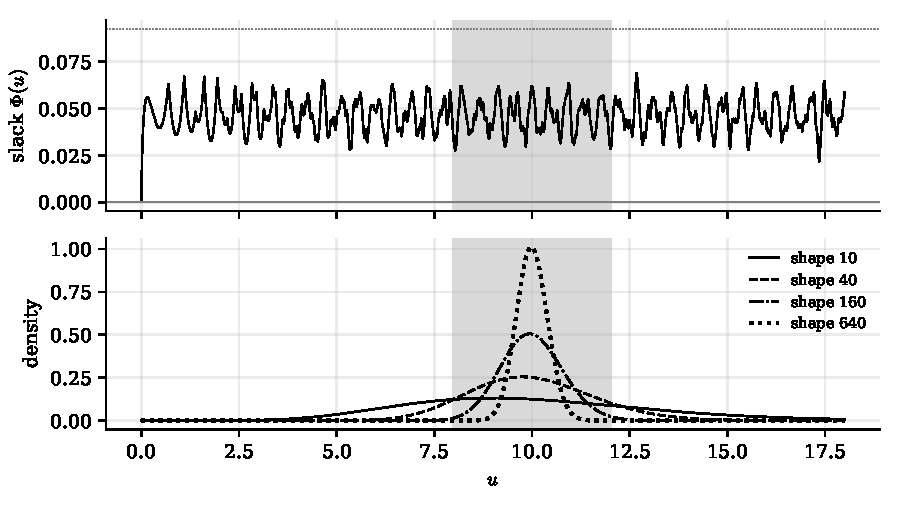
\includegraphics[width=0.95\textwidth]{fig/mq_gamma_probes.pdf}
\caption{Top: the slack $\Phi$ on $0<u\le18$, computed from the prime powers up to $10^8$, with the window $[U,\frac32U]$ for $U=8$ shaded and the line $2F_0$ dotted. Bottom: Gamma probes of mean $\frac54U$ and shapes $10$, $40$, $160$, $640$; as the shape grows the law concentrates on the window (numerically it carries $47\%$, $80\%$, $99\%$ and $99.9999\%$ of the mass).}\label{mqt:fig:probes}
\end{figure}

\subsection{Hitting times and the Wald couple}\label{mqt:sub:wald}

\begin{proposition}[Hitting time form]\label{mqt:prop:hitting}
\begin{enumerate}
\item Without hypothesis the ratio $\mathbb E[\tau e^{-\tau/8}]/\mathbb E[e^{-\tau/8}]$ equals $F_0$, and $\mathbb E\,\tau=\sum_{\gamma>0}\allowbreak2/\gamma^2$, which equals $\xi''(\frac12)/\allowbreak\xi(\frac12)=0.0462100$ (so $\mathbb E\,T=0.0231050$).
\item The following are equivalent: (a) RH; (b) $\tau$ is a generalised gamma convolution; (c) $\tau$ has the law of $\sum_{\gamma>0}e_\gamma/\lambda_\gamma$ with independent standard exponential $e_\gamma$ and positive real rates $\lambda_\gamma$; (d) $\Phi(u)\ge0$ for all $u\ge0$; (e) for every $\epsilon>0$ there are arbitrarily large $U$ with $\Phi(u)\ge-e^{\epsilon u}$ for all $u\in[U,2U]$.
\item Assume RH, let $m_\gamma$ be the multiplicity of a distinct positive ordinate $\gamma$, and let $\Gamma$ be the ordinate with $\mathbb P(\Gamma=\gamma)=m_\gamma(\lambda_\gamma+\frac18)^{-1}/F_0$, the summand selected by size biasing $\tau$ tilted at $\frac18$ (Lemma~\ref{mq:lem:sizebias}). Then $\Phi(u)=F_0\,\mathbb E[2\sin^2(\Gamma u/2)]$ for all $u\ge0$.
\end{enumerate}
\end{proposition}

\begin{proof}
(1) $-\frac d{ds}\log\mathbb E\,e^{-s\tau}=\frac d{ds}\log\xi(\frac12+\sqrt{2s})=\frac1\lambda\frac{\xi'}\xi(\frac12+\lambda)$ with $\lambda=\sqrt{2s}$; at $s=\frac18$ this is $2\frac{\xi'}\xi(1)=F_0$, and as $s\to0$ it is $\frac d{d\lambda}\frac{\xi'}\xi(\frac12+\lambda)|_0=(\log\xi)''(\frac12)$. (2) (a) $\Leftrightarrow$ (b) $\Leftrightarrow$ (c) is Proposition~\ref{prop:rigid} with $\tau=2T$; (a) $\Leftrightarrow$ (d) is Theorem~\ref{st:thm:phi}; (e) $\Rightarrow$ (a): in Lemma~\ref{st:lem:excursion}, $R=F_0-\Phi$ and $B=\sup\Re\rho-\frac12$; if $B>0$ choose $0<\epsilon<B$, then the maximum of $e^{-\epsilon u}R(u)$ on every sufficiently late dyadic interval tends to infinity, while (e) bounds it by $1+F_0e^{-\epsilon U}$ on arbitrarily late such intervals; conversely (d) implies (e) at once (windows $[U,cU]$ with any fixed $c>1$ also suffice, by Theorem~\ref{mq:thm:window}). (3) is Proposition~\ref{mq:prop:sizebias} at $a=\frac12$, with $\frac14+\gamma^2=2(\lambda_\gamma+\frac18)$.
\end{proof}

Under RH and simple zeros, $\tau$ is the first passage time of a generalised string diffusion run from its reflecting or entrance end to the absorbing level, with distinct Dirichlet eigenvalues $\lambda_\gamma$ (Kent \cite{Kent80}, \cite{Kent82}; Sections~\ref{bp:sec:kent} and~\ref{sec:ch18:kent}); Proposition~\ref{mq:prop:sizebias} does not use simplicity.

Let $\Phi_P$ be P\'olya's kernel, the even positive function with $\xi(\frac12+z)=\int_{-\infty}^\infty\Phi_P(u)e^{zu}du$, and let $X$ be the random variable with density $\Phi_P/\xi(\frac12)$, so that $\mathbb E\,e^{\lambda X}=\xi(\frac12+\lambda)/\xi(\frac12)$ for all complex $\lambda$ (equation~\eqref{eq:ch2:mgf}). Let $B$ be a Brownian motion independent of $\tau$.

\begin{theorem}[The Wald couple of $\xi$]\label{mqt:thm:wald}
\begin{enumerate}
\item Without hypothesis, $(\tau,X)$ with $\tau=2T$ independent of $X$ is a Wald couple in the sense of Definition~\ref{mw:def:wald} (the framework of Roynette and Yor \cite{RoynetteYor05}): $\mathbb E\,e^{\lambda X}\,\mathbb E\,e^{-\lambda^2\tau/2}=1$ for all real $\lambda$. Equivalently $(\varphi_X,\varphi_{B_\tau})$ is a van Dantzig pair, $\varphi_{B_\tau}(t)=1/\varphi_X(it)=\xi(\frac12)/\xi(\frac12+t)$. Consequently $\mathbb E\,X^2=\mathbb E\,\tau$, and $\mathbb E_\lambda[X]=\lambda\,\mathbb E_{\lambda^2/2}[\tau]$ for real $\lambda$, where $\mathbb E_\lambda$ is the Esscher tilt of $X$ and $\mathbb E_s[\tau]=\mathbb E[\tau e^{-s\tau}]/\mathbb E\,e^{-s\tau}$.
\item RH holds if and only if $\tau$ is a generalised gamma convolution, if and only if $\tau$ has the law of $\sum_{\gamma>0}e_\gamma/\lambda_\gamma$, if and only if $B_\tau$ has the law of $\sum_kL_k/c_k$ for some $c_k>0$ with $\sum_kc_k^{-2}<\infty$, the $L_k$ being independent standard Laplace variables (density $\frac12e^{-|x|}$); in that case the multiset of the $c_k$ is the multiset of the positive ordinates.
\item $X$ and $B_\tau$ have the same variance $\sum_{\gamma>0}2/\gamma^2$ but not the same law, without hypothesis: $\kappa_4(X)=-\kappa_4(B_\tau)=-3\,\mathrm{Var}\,\tau=-12\sum_{\gamma>0}\gamma^{-4}<0$ (conjugate terms grouped), so that $X$ is platykurtic and $B_\tau$ leptokurtic.
\end{enumerate}
\end{theorem}

\begin{proof}
(1) is Theorem~\ref{thm:ch12:idsd} together with Remark~\ref{mw:rem:waldT} (the partner exists without hypothesis, by the verification of the first zeros used there; the unconditional centre couple in precisely the doubled clock normalisation is also in Section~\ref{c:sec:wald}), and the identities follow by differentiating $\log\mathbb E\,e^{\lambda X}=-\log\mathbb E\,e^{-\lambda^2\tau/2}$ twice at $0$ and once at $\lambda$. (2) is Proposition~\ref{prop:rigid} and, for the last form, the equivalence recorded after \cite[Theorem~2.3]{KPS24} in Chapter~\ref{ch:boschA}. (3) Conditioning on $\tau$ gives $\kappa_4(B_\tau)=3\,\mathrm{Var}\,\tau>0$, since the clock is not degenerate and $\mathrm{Var}\,T=\sum_{\gamma>0}\gamma^{-4}>0$ with conjugate terms grouped, and the identity of (1) gives $\kappa_4(X)=-3\,\mathrm{Var}\,\tau<0$; both variances equal $\mathbb E\,\tau$. No hypothesis is used.
\end{proof}

The partner exists unconditionally and RH is the form of the partner (item 2); RH is not the equality in law of $X$ and $B_\tau$, which fails by item 3.

\begin{theorem}[The Esscher form of the constant, the variance and the criterion]\label{mqt:thm:esscher}
Without hypothesis, let $m(\lambda)=\mathbb E_\lambda[X]=\frac{\xi'}\xi(\frac12+\lambda)=\sum_{\gamma>0}\frac{2\lambda}{\lambda^2+\gamma^2}$ for real $\lambda$. Then
\begin{enumerate}
\item $F_0=2\,m(\tfrac12)=2\,\mathbb E_{1/2}[X]$;
\item $\mathrm{Var}\,X=m'(0)=\sum_{\gamma>0}2/\gamma^2=0.0462100$;
\item for $b>\frac12$ the Laplace transform of the slack is the divided difference of $\lambda\,m(\lambda)$,
\[
\hat\Phi(b)=\int_0^\infty e^{-bu}\Phi(u)\,du=\frac{b\,m(b)-\frac12m(\frac12)}{b\,(b^2-\frac14)},
\]
where $m(b)=\frac1{b+\frac12}+\frac1{b-\frac12}-\frac12\log\pi+\frac12\psi(\frac14+\frac b2)-\sum_n\Lambda(n)n^{-1/2-b}$.
\end{enumerate}
Consequently (Theorem~\ref{st:thm:cm}) RH holds if and only if this function is completely monotone on $(\frac12,\infty)$.
\end{theorem}

\begin{proof}
(1) $m(\frac12)=\frac{\xi'}\xi(1)=1+\frac{\gamma_E}2-\frac12\log4\pi$. (2) The second cumulant of $X$ is the coefficient of $\lambda^2/2$ in $\log\xi(\frac12+\lambda)$. (3) With $a=\frac12$ the paired explicit formula gives $\Phi(u)=\sum_{\gamma>0}2(1-\cos\gamma u)/(a^2+\gamma^2)$; the weights are absolutely summable and $|\Im\gamma|<\frac12$ without hypothesis, so that $e^{-bu}(1+e^{u/2})$ justifies termwise integration for $b>\frac12$, and $\hat\Phi(b)=\frac1b\sum_{\gamma>0}\frac{2\gamma^2}{(a^2+\gamma^2)(b^2+\gamma^2)}=\frac{b\,m(b)-a\,m(a)}{b(b^2-a^2)}$, the last equality by subtracting $2a^2/(a^2+\gamma^2)$ from $2b^2/(b^2+\gamma^2)$ term by term; this is the formula of Theorem~\ref{st:thm:cm} (equation~\eqref{st:eq:phihat}) with $F_0=2m(\frac12)$. The expression for $m(b)$ is the logarithmic derivative of $\xi$ written with $\xi'/\xi(s)=\frac1s+\frac1{s-1}-\frac12\log\pi+\frac12\psi(\frac s2)+\frac{\zeta'}\zeta(s)$ at $s=\frac12+b$. The equivalence is Theorem~\ref{st:thm:cm}; no window lemma is needed.
\end{proof}

The identities (1) to (3) are known in substance (the expectation $b_1=F_0/2$ of the basepoint variable in Chapter~\ref{ch:basepoint}; the Laplace transform of Theorem~\ref{st:thm:cm}); what is added is the Esscher reading and the divided difference form of the criterion.

\begin{remark}[Observation]
Computed from P\'olya's density at 45 digits: $2\,\mathbb E_{1/2}[X]$, $2\frac{\xi'}\xi(1)$ and a numerical derivative of $\log\xi$ all equal $0.0461914179322$ (largest difference $5.5\cdot10^{-48}$), $\mathrm{Var}\,X=0.04620998623$, and the Laplace side of Theorem~\ref{mqt:thm:esscher}(3) equals the closed form to within $1.7\cdot10^{-46}$ at $b=1,2,5$. The standard deviation of $X$ is $0.21497$ and the density at $0$ is $1.797$ against $1.856$ for the normal law of the same variance (Figure~\ref{mqt:fig:wald}).
\end{remark}

\begin{figure}[htbp]
\centering
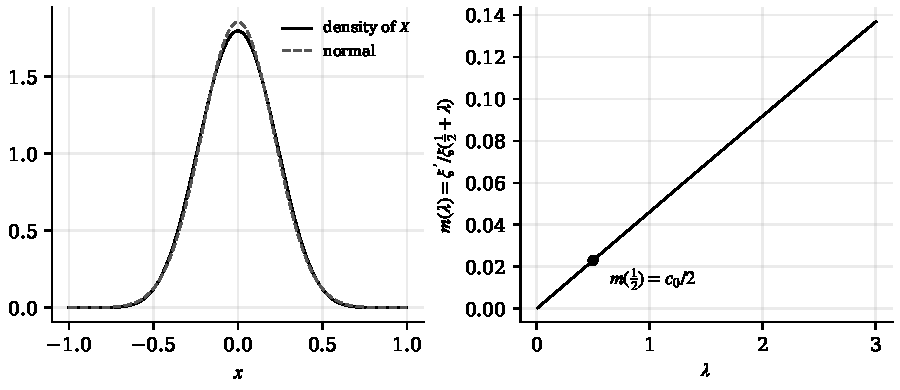
\includegraphics[width=0.95\textwidth]{fig/mq_wald_couple.pdf}
\caption{Left: the density of the P\'olya variable $X$, the first member of the Wald couple, with the normal density of the same variance $\sum2/\gamma^2=0.04621$ (dashed). Right: its Esscher mean $m(\lambda)=\xi'/\xi(\frac12+\lambda)$; the value at $\lambda=\frac12$ is half the constant $F_0$.}\label{mqt:fig:wald}
\end{figure}

\paragraph{The family and the theta kernel.} For a real primitive nonprincipal character $\chi$ of conductor $f$ the completed function $\Xi_\chi(z)=\xi_\chi(\frac12+z)$ is entire and even (the root number is $1$). Let $K_\chi$ be the even function with $\Xi_\chi(z)=\int K_\chi(u)e^{zu}du$, obtained from the theta series $\sum_n\chi(n)e^{-\pi n^2x/f}$ for $\chi$ even and $\sum_nn\chi(n)e^{-\pi n^2x/f}$ for $\chi$ odd. By the uniqueness of the bilateral Laplace transform, $\Xi_\chi/\Xi_\chi(0)$ is the moment generating function of a random variable $X_\chi$ if and only if $K_\chi\ge0$ (the density is then $K_\chi/\Xi_\chi(0)$, with $\Xi_\chi(0)=\xi_\chi(\frac12)>0$); in that case $\Xi_\chi(\lambda)=\int K_\chi e^{\lambda u}du>0$ for every real $\lambda$, so that $\xi_\chi$ has no real zero in the strip, which is the classical use of a positive theta kernel to exclude real zeros. The converse reading is not available: that $K_\chi$ fails to be nonnegative says only that $X_\chi$ does not exist, and says nothing about zeros. Nor does a one sided bound for a signed combination of Riesz means, such as $R_{q,d}$, give the existence of the clocks of its four members: Landau's theorem controls only the net multiplicity (Proposition~\ref{mq:prop:onesided}), and GRH for $\chi$ is the form of its clock and not its existence; an unconditional clock for each character would need its own proof. For the principal character the pole removing polynomial and the P\'olya kernel are used instead. Under GRH the two sided decomposition into $2\sin^2$ and $2\cos^2$ terms is Proposition~\ref{mql:prop:twosided}, and the theta kernel test for the choice of $(q,d)$ is in Section~\ref{mql:sub:choice}.

\subsection{The Stieltjes fraction at the centre}\label{mqt:sub:stieltjes}

Let $S(s)=\sum_{\gamma>0}(s+\gamma^2/2)^{-1}$, which is $\frac d{ds}\log\xi(\frac12+\sqrt{2s})$, and expand it at $s=0$ as a Stieltjes continued fraction $S(s)=c_1/(1+c_2s/(1+c_3s/(1+\cdots)))$. By the equivalence (T11) of Theorem~\ref{d:thm:forms}, Proposition~\ref{c:prop:grommer} and equation~\eqref{b:eq:Sfrac}, RH holds if and only if every $c_j$ exists and is positive; the book also holds the centre Hankel minors, in a normalisation in which $S$ is expanded in $u=2s$. In the normalisation of Section~\ref{c:sec:string}, with first coefficient $m_0$ and then $c_j^{\rm book}$, the coefficients here are $c_1=2m_0$ and $c_{j+1}=2c_j^{\rm book}$ for $j\ge1$, and in particular $c_1=\mathbb E\,\tau=0.0462100$ while $m_0=c_1/2=\sum_{\gamma>0}\gamma^{-2}=0.0231050=\mathbb E\,T$.

\begin{remark}[Observation]
From the Taylor coefficients of $\log\xi$ at the centre (a Cauchy integral on $|z|=3$ at $260$ digits, followed by the Viskovatov continued fraction algorithm), the first ten coefficients are
\[
\begin{aligned}c_1,\dots,c_5&=0.0462100,\ 0.00321771,\ 0.00453929,\ 0.00246189,\ 0.00214657,\\
c_6,\dots,c_{10}&=0.00145011,\ 0.00134120,\ 0.00109316,\ 0.00112501,\ 0.00102159,\end{aligned}
\]
all positive (Figure~\ref{mqt:fig:stieltjes}). They agree with twice the book's coefficients, and over these ten values they decay more slowly than $j^{-2}$; the rate law that the book proposes is a heuristic, in Chapter~\ref{b:ch:chain}. No closed form is known.
\end{remark}

\begin{figure}[htbp]
\centering
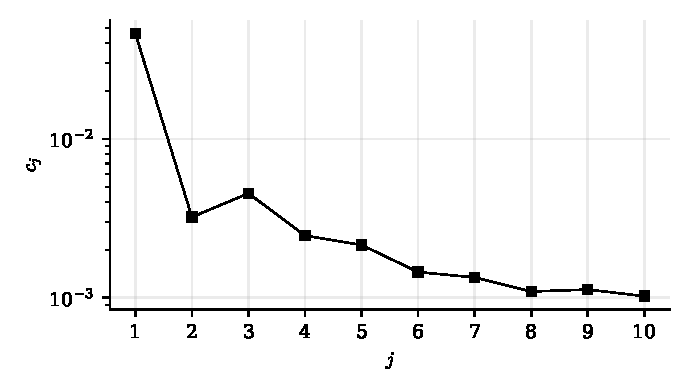
\includegraphics[width=0.85\textwidth]{fig/mq_stieltjes_c.pdf}
\caption{The first ten coefficients of the Stieltjes continued fraction of $\sum_{\gamma>0}(s+\gamma^2/2)^{-1}$ at $s=0$ (logarithmic scale), computed numerically at $260$ digits from the Taylor coefficients of $\log\xi$ at the centre. RH is the statement that all coefficients are positive.}\label{mqt:fig:stieltjes}
\end{figure}

Under RH the fraction parameters determine the masses and lengths of the string (Section~\ref{c:sec:string}); they are rational expressions in the Taylor coefficients of $\xi$ at the centre. The expansion at the centre is the one intrinsic to $\xi$. For the circle model the same fraction is classical and in closed form (Section~\ref{mqt:sub:ff}).

\subsection{The helix and the primes as extension data}\label{mqt:sub:helix}

\emph{What is a theorem.} Let $M(u,v)=\Phi(u)+\Phi(v)-\Phi(|u-v|)$. By Theorem~\ref{st:thm:pd} RH holds if and only if $M$ is positive semidefinite on $(0,\infty)$, in which case $\|f_u-f_v\|^2=2\Phi(|u-v|)$ for a curve $u\mapsto f_u$ in a Hilbert space (the helix, or screw function of Kolmogorov, von Neumann and Schoenberg, studied for $\zeta$ by Suzuki \cite{Suzuki22}; Proposition~\ref{mql:prop:differences}(3) gives the Gram matrix under RH). Near the origin the slack is elementary and has the roughness of a Brownian path with a logarithmic factor, $\Phi(u)=\frac12u\log(1/u)-0.70755\,u+o(u)$ (Proposition~\ref{mql:prop:helixprime}; the linear coefficient is $-0.7075464$, Figure~\ref{mqt:fig:slackhelix}), the factor $\log(1/u)$ coming from the Gamma factor. The quantity $M(u,u)=2\Phi(u)$ is the diagonal of the kernel, so that positivity of $M$ gives $\Phi\ge0$ and hence RH by Theorem~\ref{st:thm:phi}, and the diagonal of the kernel for $\zeta$ is the zeta analogue of (M).

\begin{figure}[htbp]
\centering
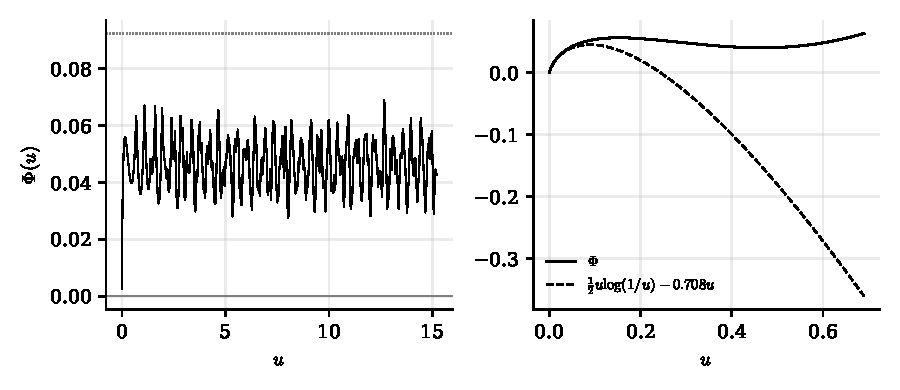
\includegraphics[width=0.95\textwidth]{fig/mq_slack_helix.pdf}
\caption{Left: the slack $\Phi$ computed from the prime powers up to $4\cdot10^6$ on $(0,15.2]$; it stays inside $[0,2F_0]$ on this range (least sampled value $0.00275$, greatest $0.0688$). Right: near $u=0$ it is elementary and behaves as $\frac12u\log(1/u)-0.7075\,u$.}\label{mqt:fig:slackhelix}
\end{figure}

The observations that follow are floating point computations on grids; positivity on a grid is a necessary condition only, and intervals reported for a weight are approximate endpoints of the discretised problem, found by bisection, and not certified. None of them is a proposition.

\begin{figure}[htbp]
\centering
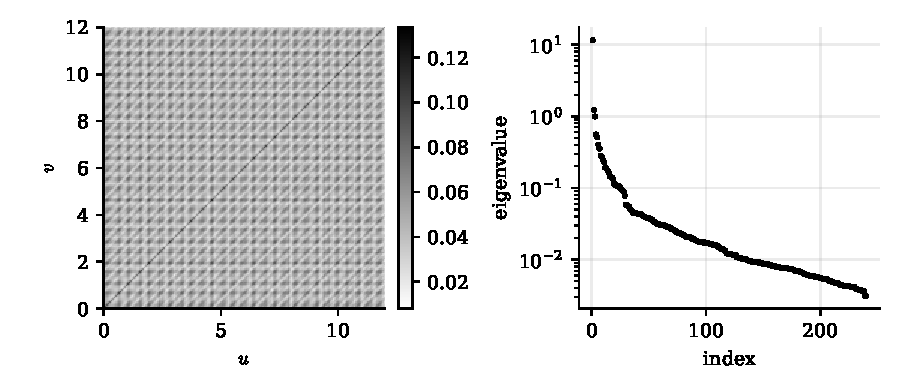
\includegraphics[width=0.95\textwidth]{fig/mq_gram_kernel.pdf}
\caption{The helix kernel $\Phi(u)+\Phi(v)-\Phi(|u-v|)$ on a grid of $240$ points of $(0,12]$, computed from the prime powers up to $4\cdot10^6$ (left), and its eigenvalues (right), the least being $3.1\cdot10^{-3}$ (numerical). Positivity of all such matrices is RH; the diagonal is the zeta analogue of (M).}\label{mqt:fig:gram}
\end{figure}

\begin{remark}[Observation: Gram matrices]
On the grid $u_i=Li/N$, $i=1,\dots,N$, the sampled matrix $M(u_i,u_j)$ has least eigenvalue $4.05\cdot10^{-3}$ for $N=150$, $2.79\cdot10^{-3}$ for $N=300$ and $1.52\cdot10^{-3}$ for $N=600$ on $(0,15]$; for $N=240$ on $(0,12]$ it is $3.13\cdot10^{-3}$ (Figure~\ref{mqt:fig:gram}).
\end{remark}

\emph{The archimedean threshold.} Write $\Phi=\Phi_\infty-P$, with $P(u)=\sum_n\allowbreak\Lambda(n)\allowbreak e^{-u/2}\allowbreak(e^u/n-1)_+$ the part from the prime powers and $\Phi_\infty$ the elementary function of Proposition~\ref{mql:prop:helixprime}, taken for all $u>0$; $\Phi_\infty$ contains the pole, the trivial zeros and the constants, that is the archimedean place. Let $M_\infty$ and $M_P$ be the kernels built from them, so that $M=M_\infty-M_P$.

\begin{remark}[Observation: Where the primes are needed]
The sampled archimedean kernel $M_\infty$ alone is positive definite on $(0,L)$ for $L\le L_N^*$, with numerical thresholds $L_N^*=0.7437$, $0.7432$ for $N=150$, $1200$ points (tolerance $-10^{-12}$), so that $L^*\approx0.743$, that is $e^{L^*}=2.10$, just past $\log2=0.693$, and has a negative eigenvalue for every larger $L$ tested, the number of negative eigenvalues at $L=0.8,\,1,\,2,\,3,\,5$ being $1,\,2,\,3,\,5,\,9$. The full kernel $M$ has least eigenvalue in $[1.2\cdot10^{-3},\,3.8\cdot10^{-3}]$ for every $L=0.20,0.22,\dots,3.20$ tested on $300$ points (Figure~\ref{mqt:fig:threshold}).
\end{remark}

The first arc of the helix, $u<\log2$, has no prime powers, so that $M=M_\infty$ there exactly; positivity there is observed only on grids. Just beyond the first prime the archimedean kernel fails, and the subtraction of the prime kernel restores positivity.

\begin{figure}[htbp]
\centering
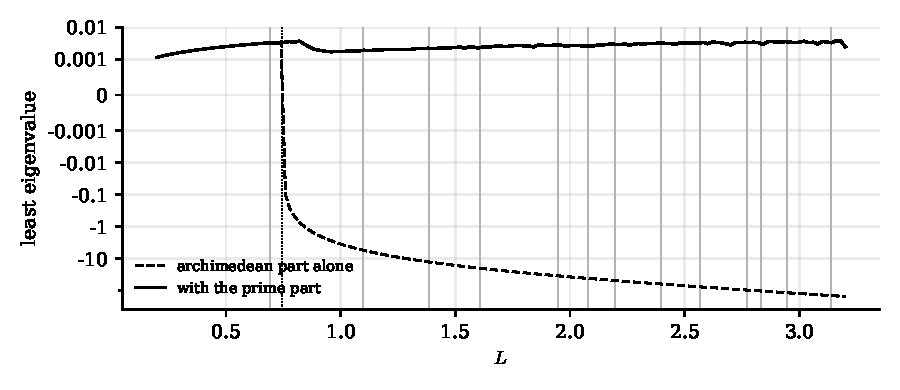
\includegraphics[width=0.95\textwidth]{fig/mq_helix_threshold.pdf}
\caption{Least eigenvalue of the kernel on $(0,L)$, on a grid of $300$ points (numerical), on a symmetric logarithmic axis. The archimedean part alone (dashed) is positive up to $L^*\approx0.743$, just past $\log2$, and then fails; with the prime part subtracted (solid) the kernel stays positive on the sampled values up to $L=3.2$. Vertical lines mark the prime powers; the dotted line is the threshold.}\label{mqt:fig:threshold}
\end{figure}

\emph{The repair is collective.} Write $K_q$ for the kernel built from the ramp $e^{-u/2}(e^u/q-1)_+$ of a point $q>1$, so that $M=M_\infty-\sum_q\Lambda(q)K_q$. $K_q$ vanishes for $L\le\log q$, and for $L>\log q$ it is indefinite, by a two point minor with points just below and just above $\log q$, where one diagonal entry is zero and the off diagonal one is not.

\begin{remark}[Observation: Repair]
On $(0,3)$, where the prime powers are $2,3,4,5,7,8,9,11,13,16,17,19$, the number of negative eigenvalues of $M_\infty-\sum_{q\le Q}\Lambda(q)K_q$ on $300$ points is $5,7,8,9,10,11,12,10,10,4,4,2,0$ as $Q$ runs through none and then these prime powers. The count rises to a maximum near $q=8$ (grid dependent) and returns to $0$ only with the last prime power below $e^L$; on $(0,4)$ it reaches $0$ at $q=53$ (Figure~\ref{mqt:fig:repair}).
\end{remark}

\begin{figure}[htbp]
\centering
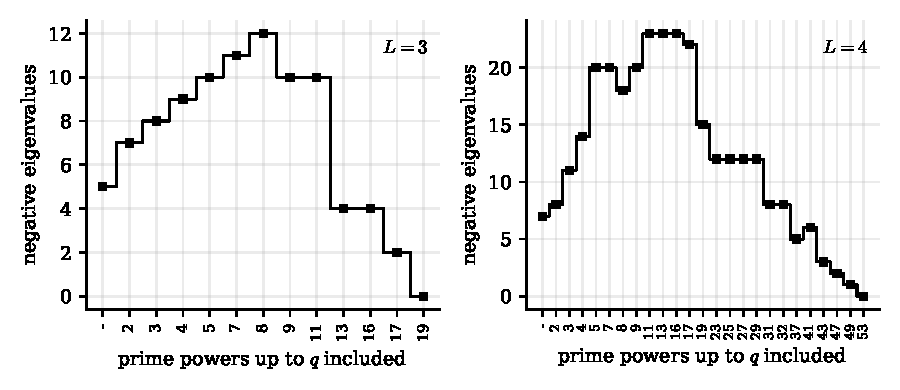
\includegraphics[width=0.95\textwidth]{fig/mq_helix_repair.pdf}
\caption{Number of negative eigenvalues of the kernel on $(0,L)$ when the prime powers up to $q$ are included, for $L=3$ and $L=4$ (numerical: a grid of $300$ points; the intermediate counts depend on the grid, the endpoints agree on the three grids tested).}\label{mqt:fig:repair}
\end{figure}

Adding prime powers makes the kernel worse before it makes it better. The rigidity of the positivity has a simple reason on the half line: changing the weight of a single prime power by $\varepsilon$ adds exactly $\varepsilon(x/q-1)_+$ to the Riesz sum, a term of size $e^{u/2}$ in $\Phi$ that violates the growth $O(u^2)$ of a function of negative type. This gives no estimate on a finite interval, where the observed rigidity reflects a least eigenvalue of order $10^{-3}$.

\emph{The funnel.} Take the positions as known and ask which weight $w$ at $\log q$ keeps the kernel positive semidefinite on $(0,L)$, the weights of the smaller prime powers being given their true values.

\begin{remark}[Observation: Admissible weights]
By bisection on the least eigenvalue ($\ge-10^{-10}$, $400$ points), the approximate admissible interval for the weight at a point $q$ on $(0,L)$ is
\begin{center}
\begin{tabular}{rrcc}
\hline
point $q$ & $L$ & admissible weights & $\Lambda(q)$\\
\hline
$2$ & $0.81$ & $[0.5731,\ 0.7275]$ & $0.69315$\\
$2$ & $1.09$ & $[0.6925,\ 0.6939]$ & \\
$3$ & $1.18$ & $[0.9473,\ 1.1729]$ & $1.09861$\\
$3$ & $1.38$ & $[1.0969,\ 1.1008]$ & \\
$4$ & $1.55$ & $[0.6850,\ 0.7072]$ & $0.69315$\\
$5$ & $1.69$ & $[1.5423,\ 1.6988]$ & $1.60944$\\
$6$ & $1.93$ & $[-0.0200,\ 0.0130]$ & $0$\\
$2.5$ & $1.05$ & $[-0.0268,\ 0.0356]$ & $0$\\
\hline
\end{tabular}
\end{center}
The interval contains the von Mangoldt weight in every case and narrows towards it over the plotted values of $L$ past $\log q$ (Figure~\ref{mqt:fig:funnel}). At a point that is not a prime power the admissible weight is confined to a small interval about zero. The endpoints of the rows for $(4,1.55)$, $(5,1.69)$ and $(2.5,1.05)$ depend on the discretisation and the tolerance.
\end{remark}

\begin{figure}[htbp]
\centering
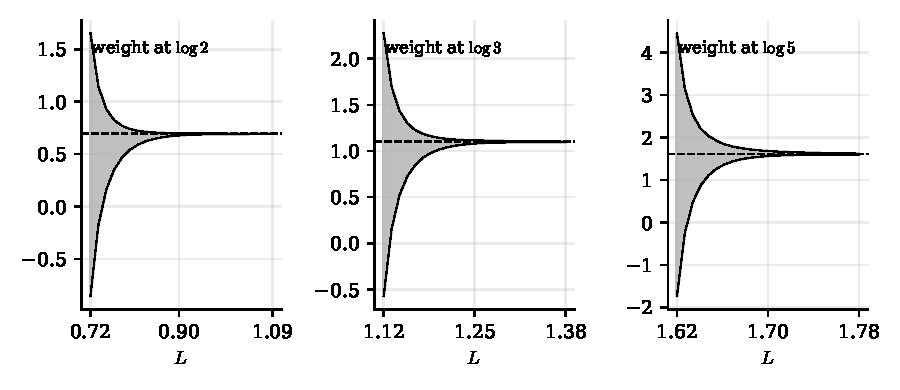
\includegraphics[width=0.95\textwidth]{fig/mq_helix_funnel.pdf}
\caption{The weights at $\log2$, $\log3$ and $\log5$ for which the helix kernel is positive semidefinite on $(0,L)$ (numerical: a grid of $400$ points), the smaller prime powers having their true weights. The admissible interval narrows towards the von Mangoldt value (dashed) over the plotted values of $L$.}\label{mqt:fig:funnel}
\end{figure}

\emph{Recovering the weights.} Optimisation over the weights at fixed candidate locations is a semidefinite programme. In an earlier numerical experiment (not reproduced here), with candidates on the quarter grid from $1.5$ to $9$ at $L=2.3$, the optimum that maximises the least eigenvalue is a positive kernel whose weights are not the von Mangoldt weights, the mass near $2$ being spread over neighbouring points, as expected from Krein's theory, by which an arc has many extensions \cite{KreinLanger14}. With candidates at the integers only, the situation is different.

\begin{remark}[Observation: The integer programme]
On $(0,3)$, with weights free at every integer $2,\dots,20$ below $e^3$ (130 grid points, least eigenvalue $7.46\cdot10^{-3}$ against $6.16\cdot10^{-3}$ for the von Mangoldt weights on the same candidates), the optimal weights for $n=2,\dots,11$ agree with $\Lambda(n)$ within $0.04$, and the agreement degrades towards $e^3$ (Figure~\ref{mqt:fig:recovered}). Maximising the least eigenvalue picks one point of a convex set, so it need not select $\Lambda$ even though $\Lambda$ is feasible; the deterioration near the right end has no demonstrated cause.
\end{remark}

\begin{figure}[htbp]
\centering
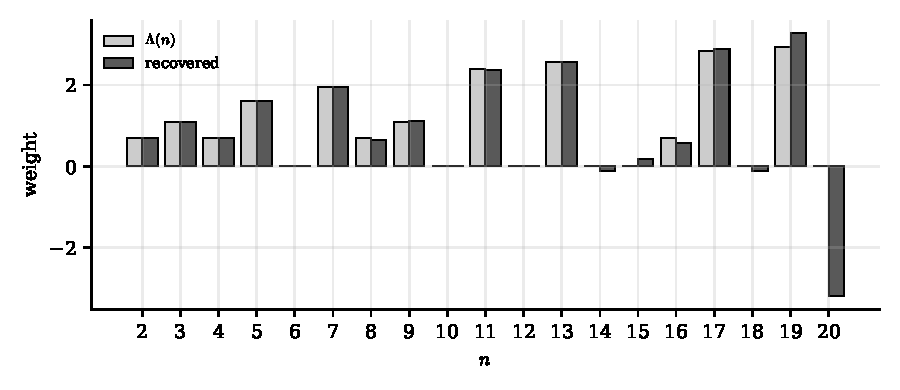
\includegraphics[width=0.95\textwidth]{fig/mq_helix_recovered.pdf}
\caption{Weights on the integers $2,\dots,20$ that maximise the least eigenvalue of the helix kernel on $(0,3)$ (numerical: a semidefinite programme on a grid of $130$ points), against the von Mangoldt function. The weights agree within $0.04$ for $n\le11$ and the agreement degrades towards $e^L$.}\label{mqt:fig:recovered}
\end{figure}

At finite $L$, on these grids, the integer supported admissible set is therefore not a point, as the funnel already shows, and any determinacy can only be a statement about the limit $L\to\infty$.

\begin{conjecture}[Determinacy, in the limit]\label{mqt:conj:determinacy}
Let $\mu=\sum_{n\ge2}w_n\delta_{\log n}$ be a real measure carried by the logarithms of the integers, with $w_n=O(\log n)$ and $P_\mu(u)=\sum_nw_ne^{-u/2}(e^u/n-1)_+$. If the kernel built from $\Phi_\infty-P_\mu$ is positive semidefinite on $(0,\infty)$, then $w_n=\Lambda(n)$ for all $n$.
\end{conjecture}

By Theorem~\ref{st:thm:pd} the converse (that the von Mangoldt weights give a positive kernel) is RH. The conjecture is of the type of Hamburger's theorem: positivity takes the place of the functional equation. The evidence is numerical, on short intervals and coarse grids, and weak. For RH and for (M) this is a formulation and not a proof: RH is the statement that the funnel at each step contains the von Mangoldt weight, equivalently that the kernel with the prescribed weights $\Lambda(n)$ is positive semidefinite on every finite set.

\emph{The helix and the integers of Part C.} The differences of the kernel in Proposition~\ref{mql:prop:differences} have an arithmetic counterpart in the formal groups of Section~\ref{mqg:sec:B4}. Figure~\ref{mqg:fig:differences} shows, for the lemniscatic curve and an inert prime $\ell$, the least $\ell$ adic valuation of the coefficients of degree $n$ of $\exp(\tilde\beta)$, with $\tilde\beta$ as in Section~\ref{mqg:sec:B4}, in the formal parameters (second difference), and of $\exp(\Delta_1\tilde\beta)$ (third difference), by exact rational arithmetic. The second difference loses about $n\ell/(\ell^2-1)$, and the third difference is integral in every degree $4,\dots,36$ computed, for $\ell=3,7,11,19$; the last is Step 1 of the proof of Theorem~\ref{mqg:thm:B4} (the unprojected case; the theorem, under our reading of (B4), concerns the projection $\beta$), and the loss of the second difference, with $n\ell/(\ell^2-1)$ as an empirical guide, is an observation.

\subsection{The finite field model}\label{mqt:sub:ff}

Over a finite field the analogues close in the cases below. For a curve over $\mathbb F_q$ with Frobenius angles $\theta_j$ (all $\theta_j\ne0$) the finite field form of the slack is Proposition~\ref{mql:prop:nakamura}: a circle of length $a=\log q$ with Frobenius holonomy, whose spectrum is a union of arithmetic progressions with the rates of that proposition, one mode for each pair $(j,k)$, including coincidences of eigenvalues. For the weighted example of Theorem~\ref{mql:thm:ffM}(3), with $q\equiv1\pmod4$, the weighted Hasse bound is the statement of the type of (M): its slack is the square of $|\sqrt q+J|/q^{1/4}$, where $J$ is the Jacobi sum, and it is nonnegative for a reason that is exactly the Weil bound; we claim nothing for other models here.

The simplest case is holonomy $-1$. The circle of length $a=\log q$ has spectrum $\lambda_k=\frac12\big((2k+1)\pi/a\big)^2$, $k\in\mathbb Z$ (two modes for each rate), and the transform of Section~\ref{mqt:sub:stieltjes} is
\[
S(s)=\frac d{ds}\log\cosh^2\Big(\frac a2\sqrt{2s}\Big)=\frac{a^2}2\,\frac{\tanh x}x,\qquad x^2=\frac{a^2s}2.
\]
\begin{proposition}[Lambert's fraction]\label{mqt:prop:lambert}
For the circle of length $a$ with holonomy $-1$ the Stieltjes fraction of $S$ at $s=0$ has
\[
c_1=\frac{a^2}2,\qquad c_{j+1}=\frac{a^2}{2(4j^2-1)}\quad(j\ge1),
\]
all positive.
\end{proposition}

\begin{proof}
Lambert's continued fraction $\tanh x=x/(1+x^2/(3+x^2/(5+\cdots)))$ gives $\tanh x/x=1/(1+\frac{x^2}3/(1+\frac{x^2}{3\cdot5}/(1+\cdots)))$ after the equivalence transformation that makes the partial denominators $1$; with $x^2=a^2s/2$ the coefficient of $s$ at stage $j$ is $\frac{a^2}2\cdot\frac1{(2j-1)(2j+1)}=\frac{a^2}{2(4j^2-1)}$. The value at $\theta=\pi$ of the mean in Proposition~\ref{mql:prop:nakamura} is $c_1$ (compare Proposition~\ref{b:prop:bessel} at Bessel index $-\frac12$ after rescaling).
\end{proof}

So for this circle the criterion of Section~\ref{mqt:sub:stieltjes} is a theorem of the eighteenth century. For $\xi$ no formula is known.

\subsection{The Thorin ladder}\label{mqt:sub:ladder}

For $\sigma>\frac12$ with $\xi(\sigma+it)\ne0$ for all real $t$, and $z>0$, put $t=\sqrt{2z}$ and
\[
\theta_\sigma(z)=\frac1{\pi t}\,\Re\Big[\frac{\xi'}\xi(\sigma+it)-\frac{\xi'}\xi(\sigma)\Big],
\]
the rung at level $\sigma$ (Section~\ref{mq:sec:ladder} states the same with $v_\alpha(y)\ge v_\alpha(0)$). Hadamard's product gives $\pi t\,\theta_\sigma(z)=\sum_\rho\Re\big[\frac1{\sigma+it-\rho}-\frac1{\sigma-\rho}\big]$, which under RH is $\pi(P_a(t)-P_a(0))$ with $a=\sigma-\frac12$ (Proposition~\ref{mqt:prop:duality}); for $\sigma>1$ it equals $C^{(\sigma-1/2)}(t)+A_\sigma(t)$, the prime part plus the archimedean part of Lemma~\ref{mq:lem:arch}; and each rung is the increment of the tilted mean $m$ along a vertical line. If $\sigma>\Theta_0=\sup\Re\rho$ (a positive gap), then for $w>0$ the transform of the rung is, as a function of $u=w^2/2$, the derivative of the negative logarithm of the compensated reciprocal at level $\sigma$,
\[
\int_0^\infty\frac{\theta_\sigma(z)}{z+w^2/2}\,dz=\frac1w\Big[\frac{\xi'}\xi(\sigma+w)-\frac{\xi'}\xi(\sigma)\Big],
\]
and the compensated reciprocal $\frac{\xi(\sigma)}{\xi(\sigma+w)}e^{w\,\xi'/\xi(\sigma)}$ is the Laplace transform in $u=w^2/2$ of a generalised gamma convolution if and only if $\theta_\sigma\ge0$. This is Theorem~\ref{pol:thm:exactlemma} with equation~\eqref{pol:eq:stieltjes}, Proposition~\ref{qt:prop:decomp} and Theorem~\ref{qt:thm:F}, and we cite them rather than reprove them.

\paragraph{What is known, and by whom.} Positivity of the rung at level $\sigma$, equivalently that $\Re\frac{\xi'}\xi(\sigma+it)$ attains its minimum in $t$ at $t=0$, is the theorem of Lagarias \cite{Lagarias}, proved there unconditionally for $\sigma>10$ and for $\sigma>\frac12$ under RH, and extended by Garunk\v{s}tis \cite{Garunkstis02} to every $\sigma$ to the right of a zero free half plane, in particular unconditionally for every $\sigma>1$ and, by a limit, for $\sigma=1$. The strict forms in the book are Propositions~\ref{bp:prop:v1min} and~\ref{bp:prop:valpha} for $\alpha\ge1$ without hypothesis and Theorem~\ref{qt:thm:Eprime} for levels above a floor. With the zero free half plane $\Re s>\frac78$ of \cite{OAI26a} (Corollary~\ref{qt:cor:floor}) every rung at a level in $(\frac78,1]$ is positive unconditionally; levels above $\Theta_0=\sup\Re\rho$ satisfy the inequality, and if $\Theta_0>\frac12$ there are failing levels arbitrarily close to it from below, while the supremum itself need not be a failing level (Proposition~\ref{mq:prop:firstrung}). If a zero $\beta_0+i\gamma_0$ with $\beta_0>\frac12$ exists then $\theta_\sigma(\gamma_0^2/2)\to-\infty$ as $\sigma\uparrow\beta_0$, so that RH is equivalent to nonnegativity of every rung at every level in $(\frac12,1)$.

\begin{remark}[Observation]
For $\sigma=0.55,\,0.75,\,1,\,2,\,3$, computed from the first $20000$ ordinates, every rung is positive (the smallest sampled value is about $10^{-7}$, near $t=0$), and the rung is largest at the first ordinate (Figure~\ref{mqt:fig:levels}).
\end{remark}

\begin{figure}[htbp]
\centering
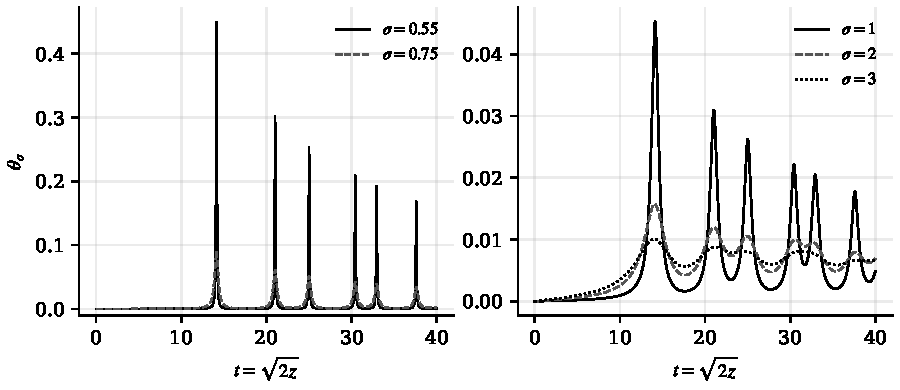
\includegraphics[width=0.95\textwidth]{fig/mq_thorin_levels.pdf}
\caption{The rungs $\theta_\sigma$ in the variable $t=\sqrt{2z}$, from $20000$ zeros, for $\sigma=0.55,0.75$ (left) and $\sigma=1,2,3$ (right): spikes at the ordinates for $\sigma$ near $\frac12$, and a smooth positive profile for $\sigma\ge1$.}\label{mqt:fig:levels}
\end{figure}

\subsection{The toy statistic for $(3,23)$}\label{mqt:sub:toy}

With $q=3$ and $d=23$ (the smallest pair meeting the congruences of Section~\ref{mq:sec:setting}) put $R_{3,23}=\mathcal G+\mathcal G_{\chi_3}-\mathcal G_{\chi_{23}}-\mathcal G_{\chi_{69}}$ as in equation~\eqref{mq:eq:R}, with $\chi_3$ and $\chi_{23}$ the Legendre symbols mod $3$ and $23$ and $\chi_{69}$ their product. The constants of equation~\eqref{mq:eq:cchi} are $c_{\chi_3}=0.1132$, $c_{\chi_{23}}=0.5693$ and $c_{\chi_{69}}=1.2389$, so that under GRH for the four functions the combination is bounded by $(F_0+c_{\chi_3}+c_{\chi_{23}}+c_{\chi_{69}})\sqrt x=1.9676\sqrt x$ up to lower order terms (Proposition~\ref{mql:prop:twosided} gives the two sided form).

\begin{remark}[Observation]
For $10\le x\le10^8$ (200000 points, with the $L'/L(1,\chi)$ at $80$ digits) $R_{3,23}(x)/\sqrt x$ lies in $[-1.060,\,1.333]$, the minimum being attained at $x=67$ and the maximum $1.333$ at $x=1354552$; from about $x=1000$ on the range is $[-0.74,1.33]$. The unsigned statistic $\mathcal G(x)/\sqrt x$ lies in $[-0.019,0.588]$. Both stay far inside the GRH envelope $1.968$ (Figure~\ref{mqt:fig:toyR}).
\end{remark}

\begin{figure}[htbp]
\centering
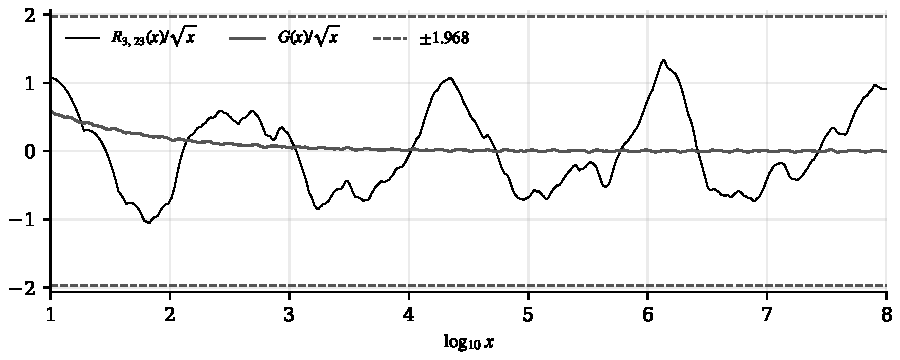
\includegraphics[width=0.95\textwidth]{fig/mq_toy_R.pdf}
\caption{The combination $R_{3,23}(x)/\sqrt x=(\mathcal G+\mathcal G_{\chi_3}-\mathcal G_{\chi_{23}}-\mathcal G_{\chi_{69}})(x)/\sqrt x$ (thin black) and $\mathcal G(x)/\sqrt x$ (thick grey) up to $10^8$; both stay far inside the leading GRH envelope $\pm1.968$ (dashed; the bound of the text has lower order terms).}\label{mqt:fig:toyR}
\end{figure}

\subsection{What the Thorin side gives, and what it does not}\label{mqt:sub:verdict}

For the zeta Riesz mean the Thorin side supplies the following equivalent formulations of RH: a one sided bound on the Riesz mean, the nonnegativity of a $2\sin^2$ transform of the Thorin measure of the zeros, the complete monotonicity of one function of $\xi'/\xi$, the existence of the clock as a generalised gamma convolution, the positivity of all Stieltjes coefficients at the centre, and the positive semidefiniteness of the helix kernel. The inequality (M) of Part A (equation~\eqref{mq:eq:M}) is a different statement: it bounds an average of translated weights with a stated error budget, with characters that can vary with the window, and its relation to the one sided bounds is that of Proposition~\ref{mq:prop:onesided} and of the conditional chain of Theorem~\ref{mq:thm:chain}, which uses the stated frame and error hypotheses; the diagonal of the helix kernel is only the zeta analogue of (M).

It does not supply a proof of (M) or of RH. The unconditional positivity statements in this language are the rungs above the floor $\frac78$ and at levels $\ge1$ (Lagarias and Garunk\v{s}tis, with the book's strict forms), the finite range $0<u\le104.86604$ of $\Phi$, and the positivity of $\hat\Phi$ over the full Abel range and of the probes in the stated range (Theorems~\ref{st:thm:abel} and~\ref{st:thm:res}). Compensated positivity at every level above $\alpha$ is equivalent to the absence of zeros in $\Re s>\alpha$; the corresponding inference from the single level $\alpha$ is open for $\xi$ (Remark~\ref{qt:rem:onelevel}). The passage from windows to the half line is proved: one sided bounds on $[Y,Y^c]$ for any fixed $c>1$ exclude zeros to the right of the exponent (Theorem~\ref{mq:thm:window}, with the signed version Theorem~\ref{mq:thm:windowcombo}). The helix computations show where the primes enter and how rigid the positivity is, but they offer no mechanism of positivity for the prime kernel. The claimed proof explained in \cite{Rub26} remains unverified here, and nothing above confirms or refutes it.

